\section{Introduction}
\label{sec:intro}
The CMS Collaboration recently published a search for new physics
in same-sign top production using events with same-sign isolated dileptons, jets, and \met~\cite{sstop}. 
In that study, as well as a closely related one~\cite{sspaper2010,ssnote2011,sspaper2011} the major
background is from \ttbar\ production, as shown in Fig.~\ref{fig:ttbar}.

\begin{figure}[htb]
\begin{center}
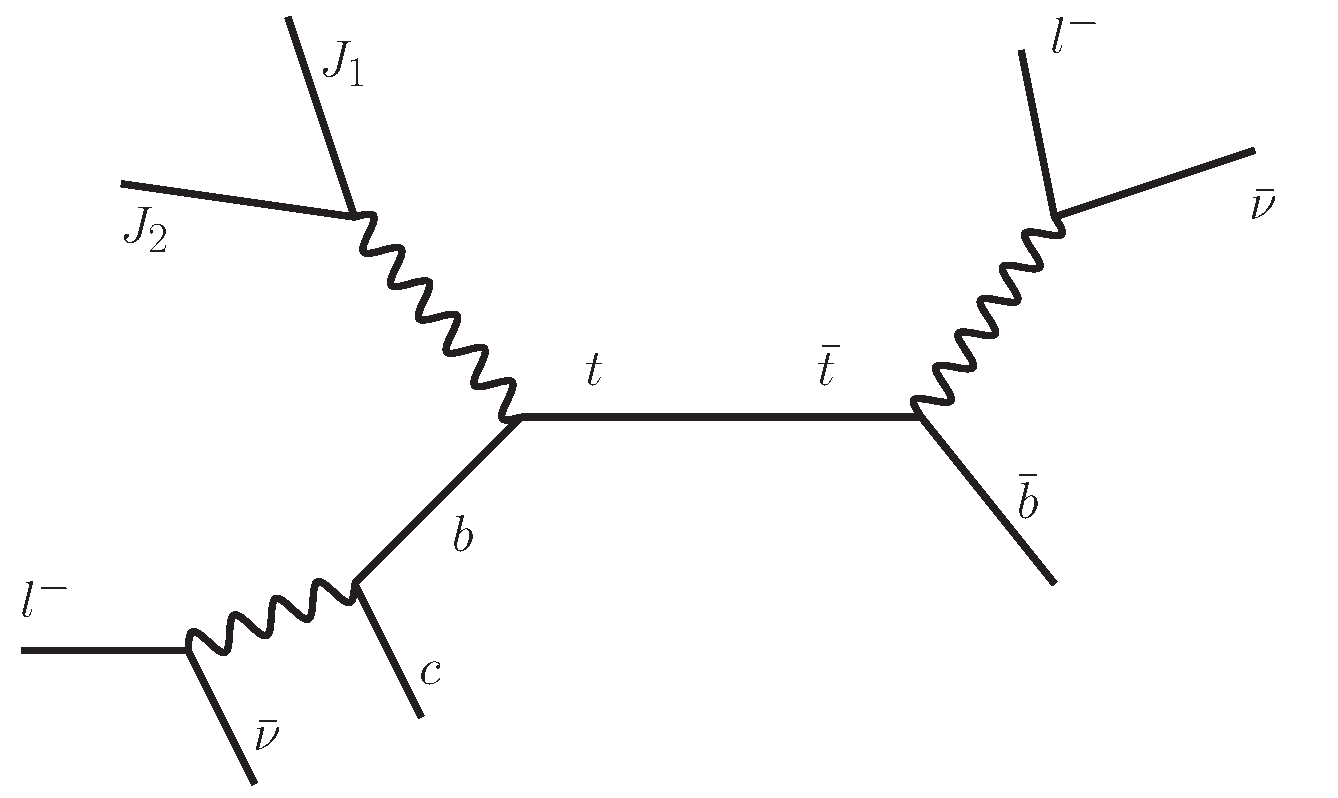
\includegraphics[width=0.6\linewidth, height=0.35\linewidth]{figs/ttbar.pdf}
\caption{ Diagram for \ttbar\ decays giving rise to same-sign dilepton final states \label{fig:ttbar}}
\end{center}
\end{figure}

The dominant source of same-sign dileptons in \ttbar\ events are produced via, $t \rightarrow W b$; where 
one of the leptons is from $W \rightarrow \ell \nu $ and the other originates from semi-leptonic $b$ decays. 
We refer to the first as ``real lepton'' and the second as ``fake lepton''.
An additional requirement on the number of $b$ jets $\geq 2$, is expected to reduce this background significantly
as a b-quark can not produce an isolated lepton and at the same time provide a b-tag.

Same-sign dileptons in association with two or more b-quarks appear naturally in many new physics scenarios.
They have been proposed as signatures of supersymmetry 
(SUSY) where heavy flavor (top or bottom) jets appear naturally~\cite{naturalness1,naturalness2,naturalness3,naturalness4},
in particular in processes with virtual stop contributions~\cite{stopVirtual,stopVirtualPRD},
those with resonant stop~\cite{stopReal},
all alternatively described with simplified models (SMS)~\cite{wacker}; 
%sbottom,gluinosbottom,
color-octet scalar production (either as sgluons in the context of SUSY~\cite{sgluons},
or non-SUSY in the context of minimal flavor violation~\cite{colorOctetScalars}); 
models of maximal flavor violation~\cite{mxflv1,mxflv2,mxflv3}; 
same-sign top quark production from flavor changing neutral currents in the top sector~\cite{fcnczprime};
pair production of $T_{5/3}$~\cite{t53};
and top compositeness~\cite{topcomp1,topcomp2,topcomp3}
%this should go into refs for susy: pair production of scalar gluons~\cite{},
among others.

All of these new physics scenarios have in common that the isolated same-sign leptons are typically decay products of on-shell W's,
thus allowing us to increase the minimum lepton $p_T$ requirements in our search to 20~\GeV, which reduces backgrounds even further.
The combination of requiring at least two $b$ jets and increasing the lepton $p_T$ threshold to 20~\GeV\ reduces the standard model backgrounds
by roughly a factor 20 over a more generic search~\cite{sspaper2010,sspaper2011}.

%In this note we perform an inclusive signature based search for events with two isolated, same-sign leptons,
%in association with at least 2 $b$ jets and \met. This generic signature should be sensitive to 
%a wide variety of new physics scenarios leading to one or more same-sign top pairs in the final state, as well as the standard model
%production of $t\bar{t}W$. In addition to the inclusive search, we thus perform several dedicated searches for a variety
%of physics scenarios, including the standard model production of $t\bar{t}W$.
 
For the purpose of this note we restrict ourselves to the $ee$, $e\mu$, and $\mu\mu$ 
final states, {\em i.e.}, we do not consider $\tau$'s, except in the case that the $\tau$ decays leptonically.

This note is organized as follows.
A brief description of the event baseline selections is given in Section~\ref{sec:eventsel},
followed by the definitions of the signal search regions in Section~\ref{sec:regions}.
Estimates of efficiencies for leptons, \met, \Ht, and b-tags, components of the event selection,
are given in Section~\ref{sec:seleff}.
We then describe methods to predict background contributions in Section~\ref{sec:bkgds},
including predictions from simulation and from data, detailed in Section~\ref{sec:datadriven}.
Results of background predictions for the defined search regions are compared with 
observed events in data in Section~\ref{sec:yields},
supported by an exclusive (disjoint) breakdown of contributions in Appendix~\ref{sec:yields_exclusive}.
Comparisons of the predicted and observed events, together with inputs relevant
to signal selection systematic uncertainties described in Section~\ref{sec:systematic}, are then used
to interpret our findings as upper limits on production of signal events beyond
the background predictions as described in Section~\ref{sec:stampCollecting}.






